%TEX TS-program = xelatex
\documentclass[11pt]{article}
\usepackage[margin=2.54cm]{geometry} % set margins to 1 inch all the way around
\usepackage{fontspec}
	\defaultfontfeatures{Ligatures=TeX}
%	\newcommand{\lmr}{\fontfamily{lmr}\selectfont} % Latin Modern Roman
%	\setmainfont{Birka LT Pro}
	\setmainfont{Kepler Std Light}
	\setsansfont[Mapping=tex-text]{Myriad Pro}
	\setmonofont[Scale=MatchLowercase]{Anonymous Pro}

% set line spacing to 1.5
\usepackage{setspace}
    \onehalfspacing 

\setlength{\parindent}{0pt} % don't indent paragraphs globally

\usepackage{titlesec}
    \titleformat{\section}{\Large\bfseries\sffamily}{\thesection}{1em}{}
    \titleformat{\subsection}{\large\bfseries\sffamily}{\thesubsection}{1em}{}

% set up indexing for all the acronyms
\usepackage{makeidx}
    \makeindex
\usepackage[acronym,toc]{glossaries}
    \makeglossaries
\usepackage{graphicx}   % this handles the non-native charts
%\usepackage[sectionbib]{chapterbib} % this handles references per chapter
% this handles the risk equation -- may not be necessary
%\usepackage{amsmath}

%\usepackage[font=sf, labelfont={sf,bf}, margin=1cm]{caption}
\usepackage[font=small]{caption}
\PassOptionsToPackage{hyphens}{url}\usepackage{hyperref}
\renewcommand{\UrlBreaks}{\do\/\do\a\do\b\do\c\do\d\do\e\do\f\do\g\do\h\do\i\do\j\do\k\do\l\do\m\do\n\do\o\do\p\do\q\do\r\do\s\do\t\do\u\do\v\do\w\do\x\do\y\do\z\do\A\do\B\do\C\do\D\do\E\do\F\do\G\do\H\do\I\do\J\do\K\do\L\do\M\do\N\do\O\do\P\do\Q\do\R\do\S\do\T\do\U\do\V\do\W\do\X\do\Y\do\Z} % this handles breaking URLS smartly
\usepackage{enumitem}

%\newcommand\smallcaps[1]{{\footnotesize\textbf{#1}}}
\newcommand\climatedge{ClimatEdge\texttrademark{} }
\newcommand\ce{ClimatEdge 2.0 }

\setcounter{tocdepth}{2} % table of contents include subsections
%\setlist{nolistsep}
%\pagestyle{empty}

\begin{document}
    %!TEX root=index.tex
\begin{titlepage}
    \vspace*{\fill}
    \begin{center}
        \textbf{\Large Christopher Keller}\\[1cm]
        \textit{A Big Data Approach To ClimatEdge\texttrademark{}}\\ [.5cm]
        CSC NPS Solution Leadership Institute\\ [.5cm]
        %\today
        March 28, 2014
    \end{center}
    \vspace*{\fill}
\end{titlepage}

    \tableofcontents
    \clearpage
    %!TEX root=index.tex
\newacronym{cse}{CSE}{Certified Solution Executive}
\section{Executive Summary}
\textsc{CSC's} ClimatEdge\texttrademark{}\index{ClimatEdge} offering is focused on providing probabilistic climate analytics using public government data sets. By using various algorithms, both proprietary and public, \textsc{CSC} plans to offer its customers a distinct advantage by allowing strategic business decisions to be made based on probabilistic outlooks in climate and extreme weather. Planned offerings for the general insurance industry include the probability of future tornado, hail, or flood occurrences in a particular geographic grid cell, as well as hail activity in the recent past.\\

This paper focuses on contrasting the tornado and flood offerings with respect to the attributes associated with big data: velocity, volume, and variety. The hail offering is similar enough in variety to tornado and in volume to flood, that analyzing it separately does not add further insights or value. The computation of tornado probabilities involves running a published algorithm against a relatively small amount of structured data on modest hardware. In short, it does not meet the criteria for big data. Flood probabilities, on the other hand, require substantially larger and more diverse data such as newspaper reports, hydrologic data from stream gauges, and parcel information in addition to rainfall and other climate data. In contrast to the tornado analytic, it does meet several criteria for big data. The minimal platform capable of delivering the tornado probabilities is not capable of offering flood probabilities. Without an investment in big data technology and expertise, the range of ClimatEdge\index{ClimatEdge} offerings will be limited.\\

Next, a reference framework implementation is presented that will allow tornado, flood, and future ClimatEdge\index{ClimatEdge} offerings to scale in processing both large and complex data sets, thus enabling a wider variety of business cases to be developed into offerings. The most important framework characteristics are flexibility in implementation technologies and a loose coupling between the layers. There does not exist a single application or technology capable of addressing every offering scenario, therefore a collection of specific technologies that can be integrated together is presented. As technologies evolve, the goal is to be able to replace any one piece of technology without overly affecting the other layers.\\

Finally, three future research ideas around the processing of large data sets are presented. The first relies on a data owner enabling programatic access, but not necessarily analysis, to the data.  The second option focuses on the possible legal implications of results derived from cloning any data sets to local storage. Finally, an approach based on moving the analysis to the provider data center is explored. Each approach has both advantages and disadvantages and is suitable for further research within \textsc{CSC} or as a follow on \gls{cse} thesis.
    %!TEX root=index.tex
\newacronym{merra}{MERRA}{Modern-Era Retrospective Analysis for Research and Applications}
\newacronym{html}{HTML}{Hyper Text Markup Language}
\newacronym{sme}{SME}{Subject Matter Expert}
\newacronym{pdf}{PDF}{Portable Document Format}
\newacronym{noaa}{NOAA}{National Oceanic and Atmospheric Administration}
\newacronym{nasa}{NASA}{National Aeronautics and Space Administration}
\section{Introduction}
Across the globe, the big data movement is changing how meteorologists are storing and analyzing data in response to global events. For example, efforts by the Korean Meteorological Administration are underway to upgrade the ability to predict weather patterns and the severity of weather events across the South Korean peninsula. IBM is engaged in similar work in Rio de Janeiro in preparation for the 2014 summer Olympics, with goals of accurately predicting short term weather \cite{rwe}. Moving past short term predictions, what if the vast repositories of weather and climate data could be collected, stored, and analyzed to produce probabilities of catastrophic events months, not weeks, in advance?\\

In 2012, \textsc{CSC's} ClimatEdge\texttrademark{}\index{ClimatEdge} service was developed to explore the commercial potential of publicly held climate and weather data. The initial offering focused on forward looking climate reports for commodities markets. The reports were written using a cursory qualitative analysis of the NASA \gls{merra} data with commentary by subject matter experts in climate sciences. The monthly reports included Global Agriculture, Global Energy, Sugar and Soft Commodities, Grain and Oilseeds, and Energy/Natural Gas \cite{climatedgeurl}. Interviews conducted with individuals associated with the original ClimatEdge\index{ClimatEdge} offering described a number of lessons learned and decisions that led to a strategy shift to a quantitative product for the next version [personal communication, 2013]. Potential customers were less interested in commentary on qualitative analysis than originally thought. Along with other factors, the ClimatEdge\index{ClimatEdge} team made the decision to focus on quantitative analysis utilizing existing CSC sales channels.\\

During the 2012 calendar year, the United States had eleven separate weather events where losses totaled more than one billion dollars each, making it the third highest loss year due to natural catastrophes since 1980 [\textsc{CSC} communication from the \gls{noaa}, 2013]. With premiums increasingly unable to cover losses incurred from extreme weather events, the overall profitability of the insurance industry is at risk. With products such as POINT IN  and Exceed, \textsc{CSC} has significant sales inroads with the general insurance industry \cite{point_in} \cite{exceed}. With established channels, the general insurance industry became a prime target for the second version of ClimatEdge\index{ClimatEdge}.\\

In order to understand offerings for general insurance, the business model must be explored. The following equation can be applied to the general insurance industry: 
\begin{equation*}
    Risk = Impact \cdot Probability
\end{equation*}
\textsc{CSC} recognized that without a substantial quantitative update, ClimatEdge\index{ClimatEdge} could not address the probability of events occurring, thus the overall risk could not be established. With a wealth of publicly available climate data from agencies such as \gls{noaa} and the \gls{nasa}, \textsc{CSC} realized a business opportunity existed. A ClimatEdge\index{ClimatEdge} offering based on quantitative analysis of publicly available data targeted towards minimizing risk for the general insurance industry would be a natural fit. The next step was to develop a technical approach to retrieving, storing, and analyzing the wealth of available data. 
\subsection{Hypothesis}
Without investing in and developing a scalable solution for big data \index{big data} storage and analytics, ClimatEdge\index{ClimatEdge} offerings will be limited to markets served by either qualitative analysis or quantitative analysis against small well-structured data sets. In order to analyze the larger and more structurally complex climate data sets, a framework of scalable technologies will need to be developed that can address both simple and complex offerings of any size. With the proper framework in place, \textsc{CSC} can offer solutions derived from analytics on data having one or more of the following big data characteristics: velocity, volume, or variety to an ever increasing number of industries.\\
 
Two contrasting ClimatEdge offerings will be explored that illustrate the different requirements necessary to store and analyze the requisite climate data. The first offering is shown to not be representative of a big data problem and is solvable by simple technology. The second offering has all the characteristics of a problem in need of a big solution. A flexible framework is then proposed that illustrates how to store and process larger and more complex data sets, such as those seen in the second offering.
\subsection{Offerings}
The large number of severe weather events in 2012, such as tornados, floods, and other natural catastrophes, caused \$160 billion dollars worth of damage in the United States \cite{stalder}. This is near the total of the previous ten years combined. Throughout that same ten year period, insured losses totaled over \$65 billion. Tornados, while a worldwide phenomenon, occur with greater frequency in the United States due to the meeting of cold Canadian air with low-level moisture from the Gulf of Mexico. Losses from these severe storms alone have accounted for more than half of all insured catastrophe losses since 1990 \cite{lloyds}. Several presentations at the Extreme Weather Congress in January 2013 focused on flooding as a prime source of damage. In the United States, floods are the most common natural disaster and average about six billion in damages each year and while the National Flood Insurance Program provides limited coverage to homeowners and businesses that qualify, a sizable secondary insurance market exists \cite{hope}. Globally, floods rank only behind earthquakes as the world's costliest natural disasters \cite{li}. \textsc{CSC's} Data Services group, in conjunction with industry analysts and other internal groups, has identified several opportunities in which an updated ClimatEdge\index{ClimatEdge} offering can benefit the general insurance industry [personal communication, 2013]:
\begin{itemize}
    \item probability of future tornado occurrence
    \item probability of future hail occurrence \& recent forensics
    \item probability of future global and domestic flood occurrence
\end{itemize}
This paper examines the tornado and flood probability analytics as having contrasting requirements at either end of the attribute scale associated with big data. The analytics necessary for producing a hail offering are an offshoot of the tornado algorithm and the data sets required are also similar in complexity to the tornado sets. A detailed examination of the hail offering would therefore, not yield significant additional insight as compared to tornado and flood offerings.
    %!TEX root=index.tex

\newacronym{ncdc}{NCDC}{National Climatic Data Center}
\newacronym{soi}{SOI}{Southern Oscillation Index}
\newacronym{tvs}{TVS}{National Tornado Vortex Signature}
\newacronym{mda}{MDA}{National Mesoscyclone Detection Algorithm}

\section{Case Study: Tornado}

CNK - why am i focusing on tornado (dan provides research). There are some hail modesl on the market for catosptrophic risk 

A primary carrier of property and casualty insurance would potentially be very interested in knowing the probability of tornado occurrence in geographical areas in which they have a large customer base. There are two months in the year which kick off tornado season in the United States: the warm season starting in March, and the cold season starting in November. Having accurate predictions of weekly seasonal tornado counts, months in advance, would constitute a significant business advantage over competitors. There are two specific business cases for the property carrier to focus on:
\begin{itemize}
    \item an actuary who will use the historical year-to-year probability and future counts to create overlays based on parcel level policy and claims data on a 50km x 50km geographical grid
    \item an underwriter who will use actuarial information to create the appropriate terms and rates offering for their customers that maximizes revenues at the lowest risk level
\end{itemize}

CNK analyst said underwriter is better than actuary

A working group, consisting of Dr. Christopher Anderson, Dr. Dan Walker, and myself, has determined that the data layer for tornado prediction should contain the following data sets [unpublished, 2013]:
\begin{itemize}
    \item 1 MB of \gls{soi} historical archives \cite{bom}
    \item 100 MB of \gls{tvs} and \gls{mda} \cite{hdss}
    \item 1.5 TB of \gls{ncdc} historical tornado report \cite{ncdc}
\end{itemize}
All of this data is in the public domain and freely available to anyone that has the resources to store and analyze it. As mentioned in chapter one, currently CSC uses only the summary information provided by Giovanni in the \climatedge product. While Giovanni has the advantage of requiring no local computational resources, it represents the tip of the proverbial data iceberg and does not help in quantitative prediction. Dr. Anderson has speculated that there exist variables stored within the three dimensional \gls{merra} archives that can be utilized to further improve prediction. This additional data would be:
\begin{itemize}
    \item 2.5 TB of \gls{merra} 3D historical \cite{mdisc}
\end{itemize}
The entirety of the data sets listed above can vary in size from a few hundred gigabytes to a few terabytes just for the raw data. In order to quantitatively process this data, we need a service platform capable of performing the following operational layers:
\begin{itemize}
	\item retrieving data updates
	\item storing and indexing for optimal retrieval
	\item data discovery and analytics
	\item presenting real-time and offline results
\end{itemize}
We can represent each layer graphically, building on the layer to its left. 
\begin{figure}[htp]
    \centering
%    \caption*{Data flow by layer}
    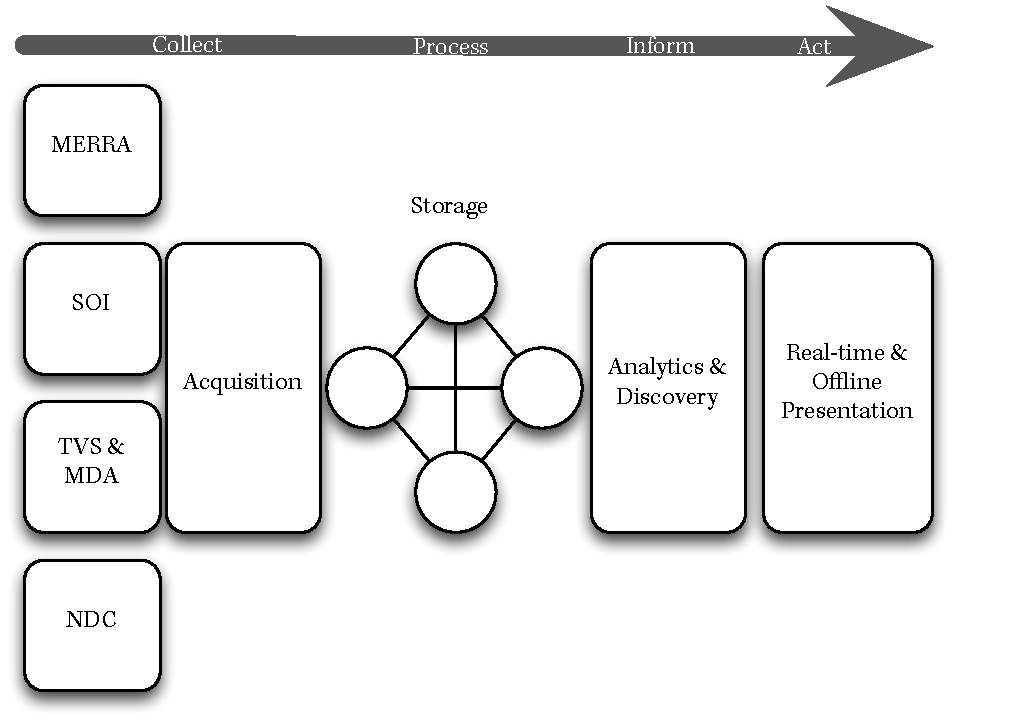
\includegraphics[scale=.75]{dataflow}
\end{figure}

\subsection{Data Acquisition}
As all the data is freely available via standard HTTP requests, we simply need to put together a framework consisting of a repeatable process that polls each website for newly published data and retrieves it. If necessary, the framework can check with the data store to confirm what's new and what's not. Putting together such a framework is a relatively simple systems integration and development task and has plenty of prior art across the industry. I'd recommend the following components:
\begin{itemize}
	\item Three Linux instances to handle retrieval, monitoring, and hosting the source code repository, respectively.
	\item A continuous integration tool, Jenkins or similar, for continually monitoring and notifying the success or failure of the retrieval processes (one per data set). Jenkins will also serve as the means to deploy the most recent code from the code repository onto the server handling the retrieval process. Jenkins is open source and used commonly across the industry for this purpose, resulting in an easily hirable skill set \cite{jenkins}.
	\item A repeatable method, such as Cron, to check and retrieve updated data sets at well defined publication intervals. Jenkins will monitor the success or failure of the cron jobs and notify as needed.
	\item Developed code that contacts each web server and pulls down only the most recent data. If the data sets do not offer a simple means of determining what's recent, this code can query the data store so that it's aware of the last stored data. While we need unique code for each data set, the process of determining what's new and retrieving the code should be very similar across all the data sets. It's likely there will a reusable common library of functionality across each specific implementation. This development is likely to be done in a scriptable environment such as Python or Perl. The languages offer an excellent tradeoff between simplicity, flexibility, and execution speed.
\end{itemize}

\subsection{Storing and Indexing}
Once the data has arrived on the local system, it needs to processed and inserted into the data store. This layer is the heart of any service offering. The data store must have the following characteristics:
\begin{itemize}
	\item Not inherently possess a single point of failure
	\item Horizontally scale (as linearly as possible) in storage and performance
	\item support realtime and batch analytics
\end{itemize}
There exist several technologies in the top level Apache Hadoop project, one being Cassandra\index{Cassandra}, which fulfill the requirements listed above\cite{cassandra}. There of competing technologies from commercial vendors like EMC, IBM, Intel, SAS, and Oracle, just to name a few, who have similar technologies designed to store and index vast amounts of data. Regardless of technology, within the data store implementation, we can use the following generic key-value model for storing any piece of climate data.
\begin{table}[htbp]
	\caption*{Climate Data Model}
	\centering
	\begin{tabular}{l l}
		\hline
		Key & Value \\ [0.5ex]
		%heading
		\hline
		meta-data & what the measurement represents, i.e., total precipitation or soil moisture\\
		time & time and date of measurement in UTC, i.e., YYYY-MM-DD HH:MM:SS\\
		coordinates & geographic location in latitude and longitude, i.e. -90.0 to 90.0 and -180.0 to 180.0\\
		value & measurement value, i.e. 0.000052977\\
		\hline
	\end{tabular}
\end{table}
With this simple structure and specific materialized views \index{materialized views}\cite{materialized_views}, we enable analytics based on any combination of the following searches: temporal, geospatial, or by meta-data.

\subsection{Discovery and Analytics}
The technology behind big data storage is really only interesting to engineers. What we want are the results of the stored data analysis. For tornado prediction, the specific analytic we'd produce is a 50km x50km (based on input data granularity) geo-spatial grid of predictions of the probability of tornado occurrences expressed as a Poisson distribution [unpublished, 2013]. This analytic would be computed twice a year in the months leading up to the tornado season in order to give the carriers enough time to react to the data.

\subsection{Presentation}
It's possible to represent the resulting Poisson distribution in a number of ways, either textually or graphically. While an interactive \gls{html} geographical map may best present the results for human consumption, the goal should be to get the information into a system capable of overlaying it with parcel and policy data so as to present a complete picture for decision making. CSC has a policy administration tool for insurance carriers known as POINT IN \cite{point_in}. This product is widely used, making it an ideal platform to ingest the results of our predictive analytics as serialized XML containing the Poisson probabilities for each geographical grid.\\

At this point, we have a fully automated platform capable of generating predictive analytics twice a year and delivering those results electronically into an industry standard administration platform. With the future tornado probabilities by grid location, combined with the parcel and policy information, the insurance carriers now have ability to make fundamental business decisions such as: do we have enough funds to cover expected losses, do we renew policies for high probability areas, is predicted income balanced against probable risk, as well as giving another data point against fraudulent damage claims. 

%\begingroup
    % this removes the chapter title for the in-chapter bibliography
%    \renewcommand{\chapter}[2]{}% for other classes
%\renewcommand\bibname{{References}}
%\bibliographystyle{plain}
%\bibliography{chapter2}
%\endgroup
% Review of the sources: internet, C3, books, etc plus interview with the experts
	%!TEX root=index.tex
\section{Case Study: Flood}
A second business opportunity, both global and domestic flood insurance, is currently in the early planning stages within the CSC Data Services group due to its similarity to the tornado use case, making it an ideal next step for CSC.  As before, the reinsurance actuary is the preferred target:
\begin{itemize}
    \item an actuary who will use the historical year-to-year probability and future counts to create overlays based on parcel level policy and claims data
    \item an underwriter who will use actuarial information to create the appropriate terms and rates offering for their customers that maximizes revenues at the lowest risk level
\end{itemize}
The flood related data is less defined, but far more complex, than the tornado data. Again, Dr. Christopher Anderson and Dr. Dan Walker have determined that the necessary data sets to be [unpublished interview, 2013]:
\begin{itemize}
    \item NASA satellite rainfall data
    \item \gls{merra} soil moisture, atmospheric wind,  humidity, and runoff data
    \item streamflow data as available
    \item damage data from previous floods (newspaper, social media, etc) to augment streamflow
    \item satellite data of built structures and inundation
\end{itemize}
As with the tornado data, most if not all, is in the public domain and freely available.
\subsection{Objective}
The year-to-year probability of the number of floods can be expressed identically to the probability count for tornados, using a Poisson distribution. The analytics would be computed several times per year in order to account for new data and provided either on demand via a portal, an XML feed to POINT IN, or via customized  report, similar to \climatedge.
\subsection{Implementation}
Recalling the attributes of big data: velocity, volume, and variety, it becomes clear that flood prediction falls into this category more so than tornado data. It is expected that ingesting relevant newspaper and social media data will add a real time component, especially during the various flood seasons. Even without taking into account the global nature of the offering for flood prediction, the satellite rainfall and \gls{merra} data sets will be larger than the corresponding sets in tornado (mainly due to more input variables). Without even addressing existing structures, the entirety of the input data set is larger. Much of the data sets are computer published, leading to well formed input, however the media component implies significant variety in the sets.  This offering would benefit from a big data platform to handle everything from storing and indexing to analytics.

	%!TEX root=index.tex
\section{Reference Big Data Platform}
In order to quantitatively process ever increasing amounts of complex data, we need a service platform capable of performing the following operational layers:
\begin{itemize}
	\item retrieving data updates
	\item storing and indexing for optimal retrieval
	\item data discovery and analytics
	\item presenting real-time and offline results
\end{itemize}
We can represent each layer graphically, building on the layer to its left. 
\begin{figure}[htp]
    \centering
%    \caption*{Data flow by layer}
    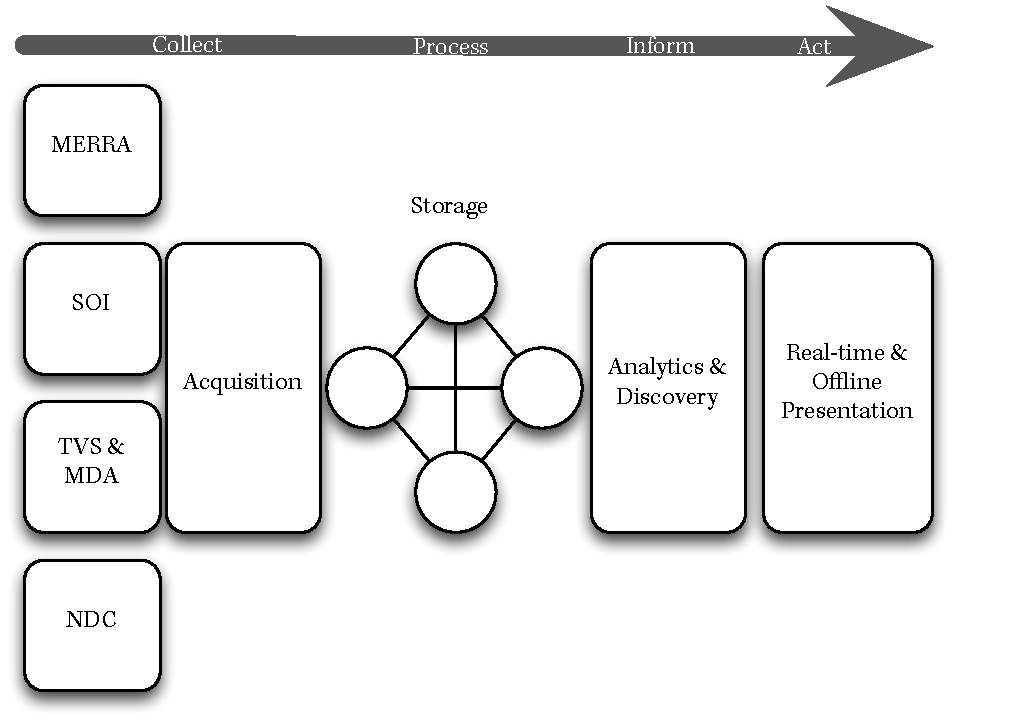
\includegraphics[scale=.75]{dataflow}
\end{figure}

\subsection{Data Acquisition}
As all the data is freely available via standard HTTP requests, we simply need to put together a framework consisting of a repeatable process that polls each website for newly published data and retrieves it. If necessary, the framework can check with the data store to confirm what's new and what's not. Putting together such a framework is a relatively simple systems integration and development task and has plenty of prior art across the industry. I'd recommend the following components:
\begin{itemize}
	\item Three Linux instances to handle retrieval, monitoring, and hosting the source code repository, respectively.
	\item A continuous integration tool, Jenkins or similar, for continually monitoring and notifying the success or failure of the retrieval processes (one per data set). Jenkins will also serve as the means to deploy the most recent code from the code repository onto the server handling the retrieval process. Jenkins is open source and used commonly across the industry for this purpose, resulting in an easily hirable skill set \cite{jenkins}.
	\item A repeatable method, such as Cron, to check and retrieve updated data sets at well defined publication intervals. Jenkins will monitor the success or failure of the cron jobs and notify as needed.
	\item Developed code that contacts each web server and pulls down only the most recent data. If the data sets do not offer a simple means of determining what's recent, this code can query the data store so that it's aware of the last stored data. While we need unique code for each data set, the process of determining what's new and retrieving the code should be very similar across all the data sets. It's likely there will a reusable common library of functionality across each specific implementation. This development is likely to be done in a scriptable environment such as Python or Perl. The languages offer an excellent tradeoff between simplicity, flexibility, and execution speed.
\end{itemize}

\subsection{Storing and Indexing}
Once the data has arrived on the local system, it needs to processed and inserted into the data store. This layer is the heart of any service offering. The data store must have the following characteristics:
\begin{itemize}
	\item Not inherently possess a single point of failure
	\item Horizontally scale (as linearly as possible) in storage and performance
	\item support realtime and batch analytics
\end{itemize}
There exist several technologies in the top level Apache Hadoop project, one being Cassandra\index{Cassandra}, which fulfill the requirements listed above\cite{cassandra}. There of competing technologies from commercial vendors like EMC, IBM, Intel, SAS, and Oracle, just to name a few, who have similar technologies designed to store and index vast amounts of data. Regardless of technology, within the data store implementation, we can use the following generic key-value model for storing any piece of climate data.
\begin{table}[htbp]
	\caption*{Climate Data Model}
	\centering
	\begin{tabular}{l l}
		\hline
		Key & Value \\ [0.5ex]
		%heading
		\hline
		meta-data & what the measurement represents, i.e., total precipitation or soil moisture\\
		time & time and date of measurement in UTC, i.e., YYYY-MM-DD HH:MM:SS\\
		coordinates & geographic location in latitude and longitude, i.e. -90.0 to 90.0 and -180.0 to 180.0\\
		value & measurement value, i.e. 0.000052977\\
		\hline
	\end{tabular}
\end{table}
With this simple structure and specific materialized views \index{materialized views}\cite{materialized_views}, we enable analytics based on any combination of the following searches: temporal, geospatial, or by meta-data.

\subsection{Discovery and Analytics}
The technology behind big data storage is really only interesting to engineers. What we want are the results of the stored data analysis. 

\subsection{Presentation}


At this point, we have a fully automated platform capable of generating predictive analytics twice a year and delivering those results electronically into an industry standard administration platform. With the future tornado probabilities by grid location, combined with the parcel and policy information, the insurance carriers now have ability to make fundamental business decisions such as: do we have enough funds to cover expected losses, do we renew policies for high probability areas, is predicted income balanced against probable risk, as well as giving another data point against fraudulent damage claims. 

%    %!TEX root=index.tex
\chapter{Big Data}

\newacronym{hdf}{HDF}{Hierarchical Data Format}
\newacronym{nosql}{NoSQL}{Not only SQL}


This can be looked at in the first paragaph of the intro


In a guest blog post, Michael Stonebraker gives four detailed definitions to the term big data\index{big data}\cite{stonebraker}. He boils it down to the same basic concepts that most of the non-technical world uses: velocity, volume, or variety. \gls{merra} data is not particularly fast moving by modern measurements: the data can be retrieved in daily (containing hourly measurements) or monthly. As far as volume goes, \gls{merra} is about two hundred terabytes since January 1979 and growing according to Dr. Daniel Walker of CSC[personal communication, 2012]. Lastly, \gls{merra} only comes in as single format known as the \gls{hdf}\cite{hdf}.\\

By Mr. Stonebraker's definition, the most applicable to ClimatEdge\texttrademark{} would be big analytics on big volumes of data. While two hundred terabytes is certainly manageable using commercially available modern hardware, it is too large to fit efficiently on a single system, thus being an excellent candidate for \gls{nosql}\index{noSQL}/big data technologies that tend to scale horizontally (scale out) rather than vertically (scale up).




%\begingroup
    % this removes the chapter title for the in-chapter bibliography
%    \renewcommand{\chapter}[2]{}% for other classes
\renewcommand\bibname{{References}}
\bibliographystyle{plain}
\bibliography{chapter3}
%\endgroup
% Review of the sources: internet, C3, books, etc plus interview with the experts



%\cite{csc_press1}
%Obama’s victory confirmed the value of using technology and data analytics. The technology side of Obama’s campaign was organized into teams to oversee technology, digital and analytics. Engineers working for the campaign developed tools such as Dashboard, an online organizing community, and Obama’s analytics team developed The Optimizer, a tool for placing television advertisements in front of the most optimal audiences for the least amount of money.
%“The Obama campaign proved the power of big data,” says Gary Jackson, CSC’s director of Business Analytics. 
%    %!TEX root=index.tex
\chapter{Recommendations}
Recommendations (how should we proceed as a company -- this should Dan's stuff plus the pilot trial for sashi)

In the final two months of 2012, a demonstration was created by a small team of climatologists and engineers for Sashi Reddi, the head of \textsc{CSC's} Big Data and Analytics focus area, to present to the board of directors. This capability demonst




\renewcommand\bibname{{References}}
\bibliographystyle{plain}
\bibliography{chapter4}
%    %!TEX root=index.tex
\chapter{Further Research}
\renewcommand\bibname{{References}}
\bibliographystyle{plain}
\bibliography{chapter5}
% Review of the sources: internet, C3, books, etc plus interview with the experts

    %!TEX root=index.tex
\section{Appendix}
\newfontfamily{\anonymous}[Scale=MatchLowercase]{Anonymous Pro}
\lstset{ %
    language=C,                             % Code langugage
    basicstyle=\anonymous,
    tabsize=1,
    breaklines=true,
    breakatwhitespace=false,
    showstringspaces=false,
    showspaces=false,
    showtabs=false
}
Listed below is C code which processes a \gls{merra} data file and stores it within a simple SQLite database \cite{keller1}. Every data type would have a similar parser, typically written in Python for ease of development. However given the complex structure of the \gls{merra} format, combined with the size of the data set, it is reasonable to spend the time to develop it in C to gain execution speed. Processing a single day of \gls{merra} (300MB) and writing into an SQLite flat file takes approximately 20 seconds per variable with the listed code on a modern CPU. Similar code in Python was taking several hours to complete. The entire thirty-three year \gls{merra} archive would take approximately one week to ingest, running in parallel. 
 
\lstinputlisting{/Users/christopher/Documents/work/Climatalytics/prototype/source/merra/c/geo_point.h}
\hrule
\lstinputlisting{/Users/christopher/Documents/work/Climatalytics/prototype/source/merra/c/merra_regex.h}
\hrule
\lstinputlisting{/Users/christopher/Documents/work/Climatalytics/prototype/source/merra/c/merra_regex.c}
\hrule
\lstinputlisting{/Users/christopher/Documents/work/Climatalytics/prototype/source/merra/c/sql.h}
\hrule
\lstinputlisting{/Users/christopher/Documents/work/Climatalytics/prototype/source/merra/c/sql.c}
\hrule
\lstinputlisting{/Users/christopher/Documents/work/Climatalytics/prototype/source/merra/c/latlon.c}
\hrule
\lstinputlisting{/Users/christopher/Documents/work/Climatalytics/prototype/source/merra/c/main.c}
\lstset{ %
    language=Python,                             % Code langugage
    basicstyle=\anonymous,
    tabsize=1,
    breaklines=true,
    breakatwhitespace=false,
    showstringspaces=false,
    showspaces=false,
    showtabs=false
}
A simple mapreduce implementation for word counting in Python is presented below \cite{keller2}.
\lstinputlisting{/Users/christopher/Development/personal/mapreduce_python/pr.py}

    \bibliographystyle{plain}
    \bibliography{bibliography}
    \printglossaries
    \clearpage
    \addcontentsline{toc}{section}{Index}
    \printindex
\end{document} 
